\section{Background}

\subsection{ROSS}
ROSS \cite{carros} is an open source, parallel, discrete event simulation tool for modeling large scale systems.
There are multiple synchronization techniques that can be used when developing a PDES; ROSS uses the Time Warp protocol \cite{jefvir}.
ROSS has been heavily optimized and is very efficient when modeling large scale systems.
ROSS handles all of the parallelism and communication between different Logic Processes (LP's)
so all we had to focus on was writing the event scheduling and handling code.
The disadvantage of using ROSS is that it maintains our event list internally, and we are not allowed access to it during execution.

\subsection{Backstroke}
Backstroke \cite{vulthe} is a reverse-code generation tool for C++.
This makes it especially useful for developing the rollback code for our aircraft simulation. 


\begin{figure} [htd]
\centering
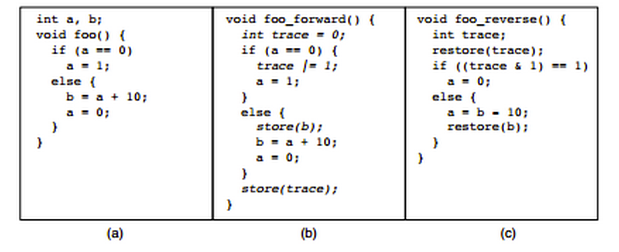
\includegraphics[width=4.2in]{/Users/chayong/Documents/project2/figs/backstroke.png}
\caption{Backstroke Code Segment}
\label{fig:backstroke}
\end{figure}


As shown in figure \ref{fig:backstroke}, in box (a), we have original method code. Using Backstroke, we achieve boxes (b), and (c), 
which constitute and forward and reverse version of this method. 
In the forward version, we store crucial state variables and in the reverse, we restore these same state variables. 
Backstroke is very useful for PDES, but it has some drawbacks. 
Backstroke does not currently support processing of loops or arrays, so we had to avoid these two constructs throughout our code
so that it would be Backstroke compatible.